\documentclass[conference]{IEEEtran}
\usepackage{amsmath,amssymb,amsfonts}
\usepackage{algorithmic}
\usepackage{graphicx}
\usepackage{textcomp}
\usepackage{xcolor}

\usepackage[numbers]{natbib}
\usepackage{hyperref}
\usepackage{url}
\def\BibTeX{{\rm B\kern-.05em{\sc i\kern-.025em b}\kern-.08em
    T\kern-.1667em\lower.7ex\hbox{E}\kern-.125emX}}
\bibliographystyle{ieeetr}


\begin{document}
\title{A Survey on Hardware Accelerators for Neural Networks}
\author{
\IEEEauthorblockN{Pierre Brosemer}
\IEEEauthorblockA{uitxj@student.kit.edu}
}

\maketitle

\begin{abstract}
This will be my Abstract in \LaTeX.
I am going to write this when I have almost finished the essay since it will probably be easier to give an overview over the topic once the full paper is finished.
The availability of efficient hardware was one of the key factors, which lead to the rise of Neural Network \cite{historyfpgas}. 
\\
\end{abstract}

\section{Introduction}
Artifical Neural Networks (more often Neural Networks) are one of the most promising technologies in the current era of computer science. Neural Networks can be deployed in an enourmous variety of categories and have shown major improvements in these categories, most prominently in Speech and Image Recognition \cite{speech_recognition1} that exceeded prior methods. The field of Artifical Intelligence covers a wide variety of concepts. This paper will mainly cover the subcategory of Deep Learning, more specifically Neural Networks, which falls under the category of Machine Learning. 
\\
Neural Networks are at it's core a very broad simplification of the biological brain consisting of many interconnected neurons, called nodes in Neural Networks. The nodes in a Neural Network are  arranged in different layers. Each node passes on a weighted function to a node in the next layer. If this value is above a certain threshhold the node will be activated. By changing the weights of each node a learning process similiar to that of their biological counterpart is simulated \cite{nn_basics}.
\begin{figure}[h]
	\caption{Typical representation of a Neural Network}
	\centering
	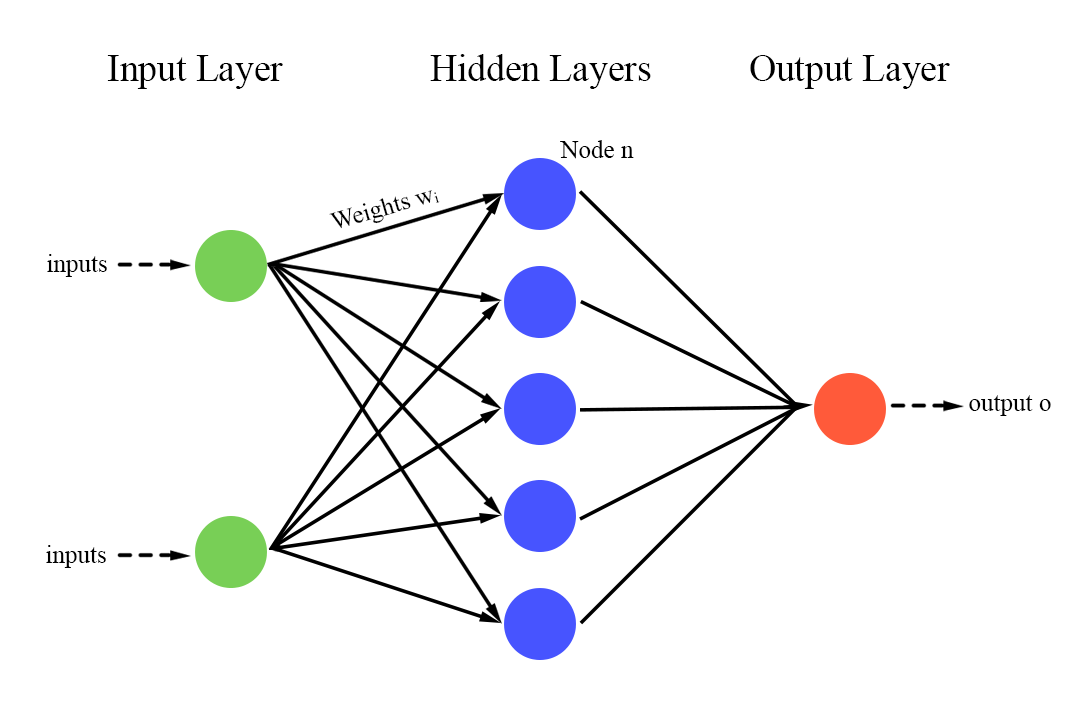
\includegraphics[width=\linewidth]{pictures/neuralnetwork.png}
\end{figure}

The development of a Neural Network consists of two different stages. Firstly a training phase where the Neural Network gets an input and compares the resulting output (prediction) with that of a real-world dataset. The error can then be incorparated into the network by changing the different weights, also called backpropagation. Secondly an inference phase, where the network get's an input and makes a prediction. The Neural Network has a larger computational demand in the training phase as more data is processed, aswell as the weights needing calibration.
\\
\\
With some Neural Networks having over 150 layers \cite{densely_network} up to billions of Multiplications can take place in a single Neural Network. The vast amount of computational power needed for training and using neural network lead to the need for specialised hardware, which contributed much to the success seen in modern day implementations. The research on hardware is still ongoing and is one of the most important topics in achieving better and faster results for Neural Networks. As a result of the timeliness of the topic this survey will only cover a status quo of the current Hardware.
\\

\section{Different Types of Hardware}
Most of Computations needed for inference and training include Matrix-Vector Products, caused by the input data being run through the network.
Furthermore  the dimension of the input data plays a key role in the amount of computation needed. Lets say a single image has 1000 pixels resulting in 1000 different data points that the Neural Network has to compute. To efficiently compute the vast amount of data fast memory accesses or inplace computations of the values is needed. Since these Calculations need to be done for the number of nodes good parallelization is needed to efficiently run Neural Networks.
\\
Hardware Accelerators for Neural Networks can be divided into 4 main classes: CPUs, GPUs, FPGAs and ASICs. The focus can be placed on the latter 3 since CPUs mostly fall short in terms of computational power for Neural Networks. 
CPUs are needed for a wide variety of tasks requiring a flexible system to execute instructions. As a result a CPU is good at executing serial instructions in parallel, resulting in a good general parallelization.
Both of the points mentioned above, that are needed for the specialised hardware for Neural Networks, are not met for CPUs. They are limited by their small amount of cores hindering the ability to parallelize the same instruction. Moreover a CPU usually works by fetching an instruction and executing it making the training and inference phase slow \cite{capra2020updated}. While working on Neural Networks CPUs are accompanied by Underutilization, achieving factors of less than 1/10 of that other alternatives \cite{nurvitadhi2016accelerating}. Nonetheless Intel is working on accelerating CPUs producing librarys for their Intel Xeon Processor \cite{intelnn}.
\\
Another point to consider is the different requirements needed for both the training and inference phase. During the inference phase certain approximasations can be made to achieve faster results, which can't be made for the training phase. This derives in some Hardware only being designed for the inference phase. 

\section{Graphics Processing Unit}
The Graphics Processing Unit (GPU) is a piece of specialised Hardware originally designed for the rendering of images in a Computer. The rendering process requires vast amounts of floating point operations resulting in the GPU having hundreds of cores with many individual caches to store the computation. To add on the GPU has more units dedicated to floating-point operations. This makes the GPU an excellent tool for working with Neural Networks since the their specifications align with those for rendering Graphics. With over thousands cores the GPU can parallelize the matrix multiplications needed for training and achieve fast training times. 
\begin{figure}[h]
	\caption{Different Layouts comparing CPU and GPU: The GPU has more cores with more individual Caches \cite{intelpic_comparison}}
	\centering
	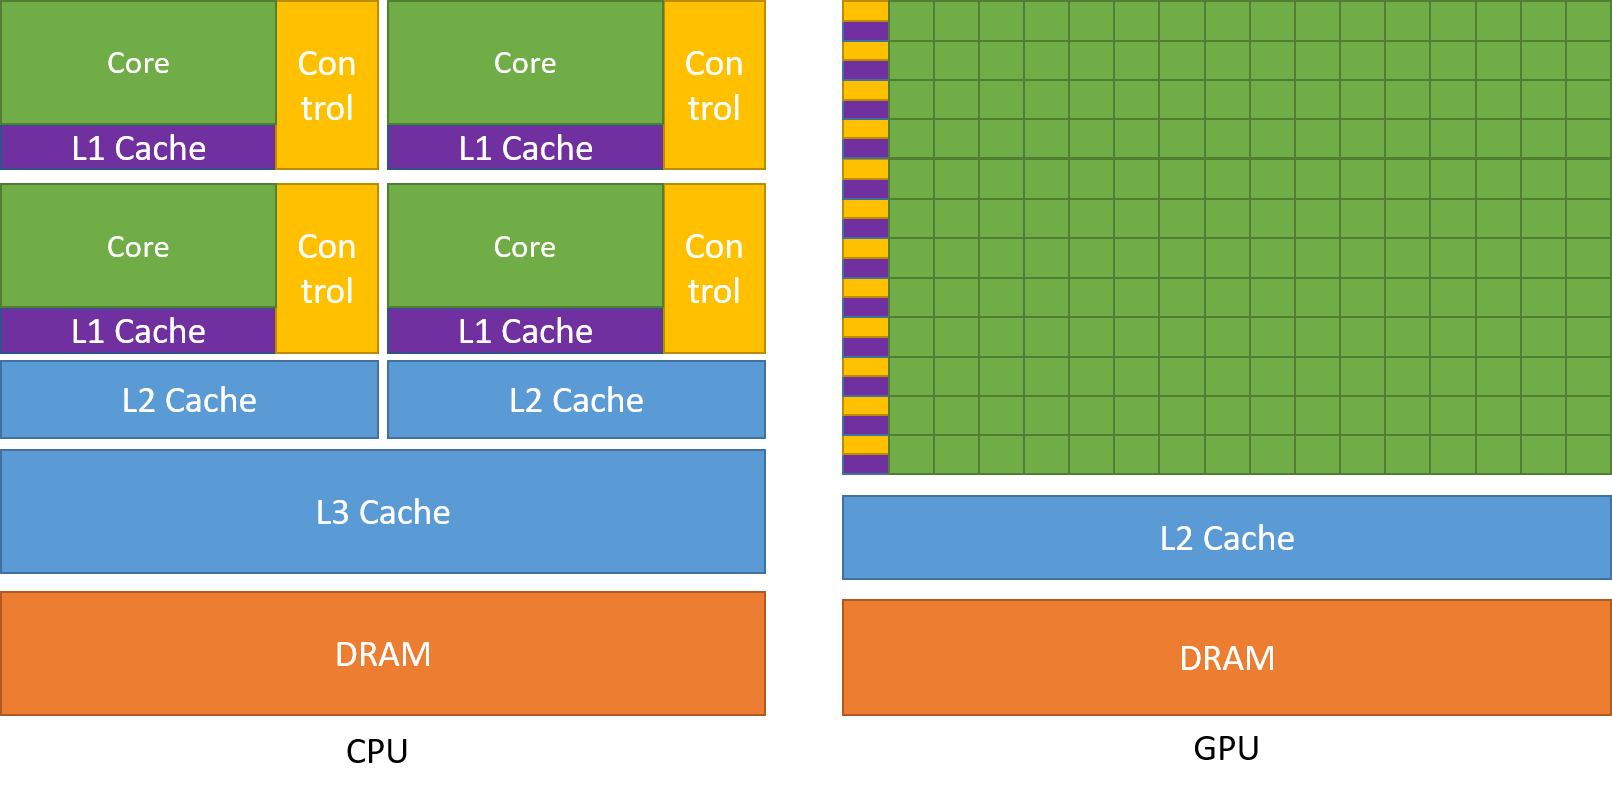
\includegraphics[width=\linewidth]{pictures/intel_comparison.png}
\end{figure}

Through this structure high memory throughput and good Execution of parallel instructions is given. Nvidia ,one of the leaders in manufactoring, is implementing the their specialised Deep Learning Units with normal cores plus additional Tensor cores \cite{nvidiav100}. Tensor Cores essentiely multiply 2 FP-16 Matrix (Floating Point 16 bit) and being able to add a third Matrix all in a single operation, performing 64 operations per clock \cite{tensorcores}. Their newest product the Nvidia A100 uses the third generation of tensor cores with better precision.
Another way GPUs accelerate is by making use of the sparsity of matrices used for calculating the different functions, more on that later.
GPUs can be seen as the most used hardware option for neural networks for general scientific usage \cite{mostusedgpu}. They are mostly used for training, but can also be used for the inference phase because of their flexible hardware structure \cite{capra2020updated}. They are specifically fast in training due to their ability to work through large amounts of data quickly (having a high memory bandwidth).

\section{Field-programmable Gate Array}
A Field-programmable Gate Array (FPGA) is an integrated circuit, which can be programmed by the customer after delivery. The concept of a unit can be configured by using Hardware Description Language (HDL). FPGAs contain logic blocks which in the process can be altered by the HDL. The logic blocks can be configured to execute complex functions or simple logical operations. FPGAs are also used as prototypes for ASICs, since their time to develop is much lower than ASICs. A big Problem for researchers working on FPGAs is the hardware-specific knowledge needed for reprogramming them after receiving the product. In recent years however a shift towards a more software-close programming can be seen. Despite the shift, writing code is can still be a challenge, because the code written for software is fundamentally different than that written for FPGAs. This also opens the door for researchers on neural networks to speed up the training and inference phase for neural networks, since working with a flexible and user-friendly framework is of advantage. The major manufacturers are Xilinix (owned by AMD) and Altera (owned by Intel) \cite{majorfpga}.
\\
FPGAs are limited by their flexibility compared to GPUs, with the different Logic Units needing reconfiguration, while the GPU tends to have individual units computing tasks. This process of reconfiguration leads to high compile times, making a process where changing algorithm designs often tedious. Nonetheless they offer better memory flow, by being able to program the data and control path. The on-chip memory, aswell as the ability to pipiline parallelize. The way neural network algorithms are coded als varies. Programming a neural network to be used on a GPU the focus is on parallelizing the work for different units, while on a FPGA the approach can be taken more to the software level by having more freedom in the underlying hardware, f.e. limiting the numerical precision \cite{gupta2015deep}.
\\

There are many different approaches of how to achieve efficient processing of Neural Networks with FPGAs. A vivid approach can be seen by Nurvitadhi et al. \cite{nurvitadhi2016accelerating} using Recurrent Neural Networks (Neural Networks that contain recurrent connections) for the inference phase. 
The FPGA is composed of a memory read unit, memory write unit and gatherings of multiple floating-point multiply-accumulate units (FMA). To accelerate matrix vector multiplications the matrix is first divided into column blocks. One FMA is assigned one column block to work on, mutiplying the elements of the input vector to the specified column. Since the unit only takes care of one column this can be done in place. Afterwards the result is given to a reduction unit, which adds the results of 2 column blocks for the concluding result. Many such FMA units are then group together to form a cluster seen in \ref{fig:fpgahw} . Similiar approaches like this with efficient dataflow and usage of fine-grained parallelism can be seen in other scientific works \cite{qiu2016going} \cite{wang2016dlau}.
\begin{figure}[h]
	\caption{A simplified Depiction showing the layout and dataflows of the above mentioned FPGA. Green Boxes represent the FMA units working in harmony to execute the Matrix operations \cite{nurvitadhi2016accelerating}.}
	\centering
	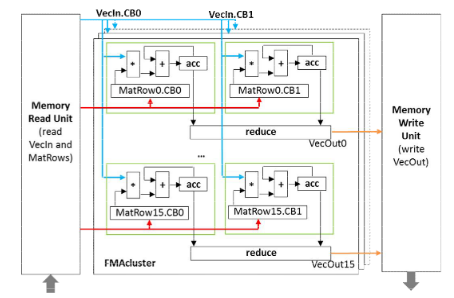
\includegraphics[width=\linewidth]{pictures/fpga_operations.png}
	\label{fig:fpgahw}
\end{figure}
\\
Microsoft found a use case for FPGAs in their datacenter for the inference phase in their Azure Cloud. The Bing ranking was accelerated by a factor of nearly 2 by using FPGAs instead of traditional Hardware \cite{putnam2014reconfigurable}. Further work was done to achieve even better performance \cite{ovtcharov2015accelerating}. A key feature of the updated hardware is the ability to support many different configurations of the hardware without having to recompile, allowing for a faster design process. The circuit is composed of many different Processing Elements aswell as Buffers. The Processing Elements can be scaled up to a margin of more units ,through their partly independent structure, to achieve faster processing times. Input data is moved from the DRAM into an input buffer. A software unit distributes the data across the Processing Elements, which perform independent operations. The results are stored in the Weight Buffer.
\\
The Buffers allow together with the Network-On-Chip to distribute data across the unit. This reduces the network traffic to and from outside of the chip, by making use of the buffers. 
\\

\section{ASIC}
An Application-specific integrated circuit (ASIC) shares many similiarities with a FPGA. The most notable difference is that while FPGAs can be reprogrammed after production, that is not the case for ASICs. They are however more efficient perfecting the hardware-specific advantages of FPGAs.
\\
Google started working on an own custom ASIC, after observing that only a 3 minutes of speech search (using Neural Networks) would double their computational capacity \cite{jouppi2017datacenter}. Making this the use-case the Hardware was therefore built specifically for the inference phase. The work became the Tensor Processing Unit (TPU). The main components of the first version included a Matrix Multiply Unit (MMU), a Unified Buffer and Accumulators. The Matrix Multiplay Unit contains 256x256 multiplier-accumulators (MACs), which perform 8-bit operations, whose results are stored in Accumulators. Many scientific works have shown that during the inference phase lower numerical precision (lower than the usual 32-bit floating point) can be used to achieve faster training times without loss of accuracy\cite{rodriguez2018lower}. This makes the Matrix Multiply Unit a good tool to process the data coming through the layers. Since the TPU is only used for inference Google implemented a Weight FIFO, which is read-only and makes accessing the weights needed in the MMU fast. The transitional results are at the end stored in the Unified Buffer. For faster processing a systolic array was used, which reduces read and write operations. Another way the hardware accelerates is by using 4-stage pipeline parallelism.
\\
The TPU V2 and V3 mainly improved 
\section{Edge Devices}

\section{Comparison Accelerators}


\section{Conclusion}

\newpage
\quad
\newpage

\bibliography{References}
\end{document}
